% -----------------------------------------------------------------------------
%   Arquivo: ./02-elementos-textuais/metodologia.tex
% -----------------------------------------------------------------------------


\chapter{Desenvolvimento}
\label{chap:desenvolvimento}

Algumas arquiteturas para resolução de problemas de otimização foram apresentadas no \autoref{chap:revisao}, em especial as que possuem alguma característica de paralelismo, seja em um único computador, utilizando \textit{multi-threading} ou em um \textit{cluster}, e que sejam baseadas em agentes. Dentre essas se destaca a arquitetura D-Optimas, objeto de estudo do presente trabalho. 

Nesta arquitetura, os agentes encapsulam metaheurísticas e interagem entre si trocando soluções através de um ambiente virtual, buscando aprender nesse ambiente a encontrar soluções de boa qualidade pra qualquer problema de otimização. O ambiente virtual, ou mundo virtual, é composto de soluções que são abrigadas em conjuntos disjuntos, chamados de regiões. O objetivo é que os agentes interajam com as regiões, e não com as soluções diretamente, ''compreendendo'', de maneira genérica, partes do espaço de busca que sejam mais ou menos interessantes. Da mesma forma, espera-se que as regiões possam apresentar uma dinâmica, podendo se fundir ou se particionar, de modo que se adaptem à geometria do espaço de busca de qualquer problema de otimização.   

A arquitetura D-Optimas foi construída baseada no modelo de atores para ser um sistema distribuído. Entretanto, alguns aspectos importantes que são inerentes à um sistema distribuído foram negligenciados na sua primeira versão, principalmente questões relacionadas ao balanceamento de carga, transparência de localidade e resiliência a falhas.

Em um sistema que cresce com o passar do tempo, com agentes produzindo soluções, regiões se fundindo, sendo criadas e se particionando, é importante que o sistema possa criar as agentes e regiões nos nós do \textit{cluster} de maneira equilibrada, de modo a não onerar nenhum nó em particular, fazendo mal uso dos recursos computacionais. A transparência de localidade também deve ser uma característica de um sistema que se propõe a resolver problemas de grande escala, sendo necessário executá-lo em um \textit{cluster} computacional, onde é difícil conhecer previamente os endereços \textit{IPs} das máquinas que executarão o experimento. A resiliência a falhas num sistema distribuído é importante pois falhas na rede são frequentes, um nó pode sair no meio da simulação, e perder as soluções que estavam nele não é aceitável, uma vez que a função objetivo pode ser complexa e custosa para se calcular.
Outro fator importante é a necessidade de uma definição mais precisa da dinâmica das regiões,  que não foi apresentada nos trabalhos anteriores.

Deste modo, neste capítulo a \autoref{sec:topologia} descreve de maneira mais detalhada os conceitos de sistemas distribuídos e os problemas encontrados na arquitetura, bem como apresenta uma nova topologia para os agentes e regiões, baseada na biblioteca \textit{akka-cluster}. A \autoref{sec:dinamica} apresenta os detalhes da dinâmica das regiões, como elas são criadas e quais as condições que permitem à elas fazer fissão e fusão. Por fim, a \autoref{sec:algoritmos} apresenta os algoritmos que foram adicionados à arquitetura, e como esse processo se deu no contexto das abstrações propostas por \citeonline{denise2014} para a generalização de metaheurísticas.

\section{Da topologia do sistema utilizando \textit{akka-cluster}}
\label{sec:topologia}
Como discutido na \autoref{sec:histBimasco}, \citeonline{pacheco} propôs uma remodelagem da arquitetura BIMASCO, utilizando o modelo de atores e o \textit{framework Akka}. Essa remodelagem deu origem à arquitetura D-Optimas, que funciona como um sistema distribuído, podendo ser executada em um \textit{cluster} com dezenas de nós e milhares de agentes. Entretanto, o autor utilizou somente os recursos mais básicos do \textit{framework}, a saber, o recurso de \textit{akka remote}. Este recurso permite que atores que executam em um processo se comuniquem com atores em outro processo.  Entretanto, só a mera comunicação entre processos não é suficiente para caracterizar um sistema como distribuído. Há três propriedades importantes para que um sistema seja considerado distribuído que estão ausentes na arquitetura D-Optimas: tolerância a falhas, balanceamento de carga e transparência de localidade. Os próximos parágrafos argumentam, baseados na literatura, a razão dessas três propriedades serem importantes e apresentam uma solução para esses três problemas, apoiada na biblioteca \textit{akka}.

Segundo \citeonline{tanenbaum}, um sistema distribuído pode ser definido da seguinte maneira:

\begin{quote}
\textit{"A distributed system is a collection of independent computers that appears to its users as a single coherent system"} \cite[p. 2]{tanenbaum}
\end{quote}

Dito isto, o autor ressalta que dois aspectos relevantes dessa definição são a característica autônoma e cooperativa dos componentes do sistema, fazendo com que o usuário, ao lidar com o sistema, perceba-o como um sistema unificado. Este aspecto em especial não está presente na primeira versão do D-Optimas. Um exemplo disso é o caso em que um dos atores supervisores falhe. Neste caso é necessário reiniciar a simulação, o que deixa claro para o usuário que os componentes não colaboram de maneira efetiva. 

Além da falta de resiliência a falhas do sistema, na versão proposta por \citeonline{pacheco} os agentes e regiões precisam saber o endereço físico uns dos outros para poderem se comunicar. É um ponto que também diverge da definição de \citeonline{tanenbaum}, uma vez que sistemas distribuídos devem ter algum nível de transparência, sendo uma das mais básicas a transparência de localidade, \textit{i.e.}, dois componentes de um sistema distribuído serem capazes de se comunicar sem saber exatamente o endereço físico de cada um \cite[p.4]{tanenbaum}.

Por fim, um último ponto que é crítico para a escalabilidade de um sistema é o balanceamento de carga. Na primeira versão 
 da arquitetura, os processos que executavam as regiões e agentes eram especializados, ou continham somente regiões, ou somente agentes. Essa decisão de projeto não contribuiu para o melhor uso dos recursos do \textit{cluster}. Enquanto os agentes fazem uso intenso do processador (\textit{CPU-bound}), para executar os algoritmos e encontrar boas soluções, as regiões fazem uso intensivo da rede (\textit{I/O-bound}), trocando mensagens entre si para decidir entre fazer fissão ou fusão. Segregar as entidades da simulação pelo seu papel pode gerar uma sobrecarga no processador de um nó, enquanto o outro nó está ocioso.
 
 Levantadas essas três deficiências, a saber, a falta de resiliência a falhas, de transparência de localidade e do balanceamento de carga entre os nós da simulação, o que se propôs inicialmente neste trabalho foi uma correção da arquitetura para abrigar essas características importantes do ponto de vista de sistemas distribuídos. Para solucionar esses três problemas o \textit{toolkit Akka} dispõe de uma funcionalidade importante, a biblioteca \textit{akka-cluster}\footnote{https://doc.akka.io/docs/akka/current/cluster-usage.html}. 
 
 Esse pacote dispõe de ferramentas uteis para a criação de um \textit{cluster} entre os atores, oferecendo algoritmos eficientes, sem ponto único de falha ou ponto único de sobrecarga. As principais ferramentas utilizadas neste trabalho é a descoberta de novos membros, detecção de falha, e eleição de líder, persistência, migração e transparência de localidade. A explicação detalhada da implementação de cada um desses conceitos pode ser encontrada na documentação da biblioteca, e por isso não serão abordados aqui. A seguir será abordado como esses mecanismos foram utilizados para construir a arquitetura e como eles facilitam a abordagem dos problemas apresentados.
 
 \begin{figure}
     \centering
     \caption{Nova organização dos atores da arquitetura D-Optimas.}
     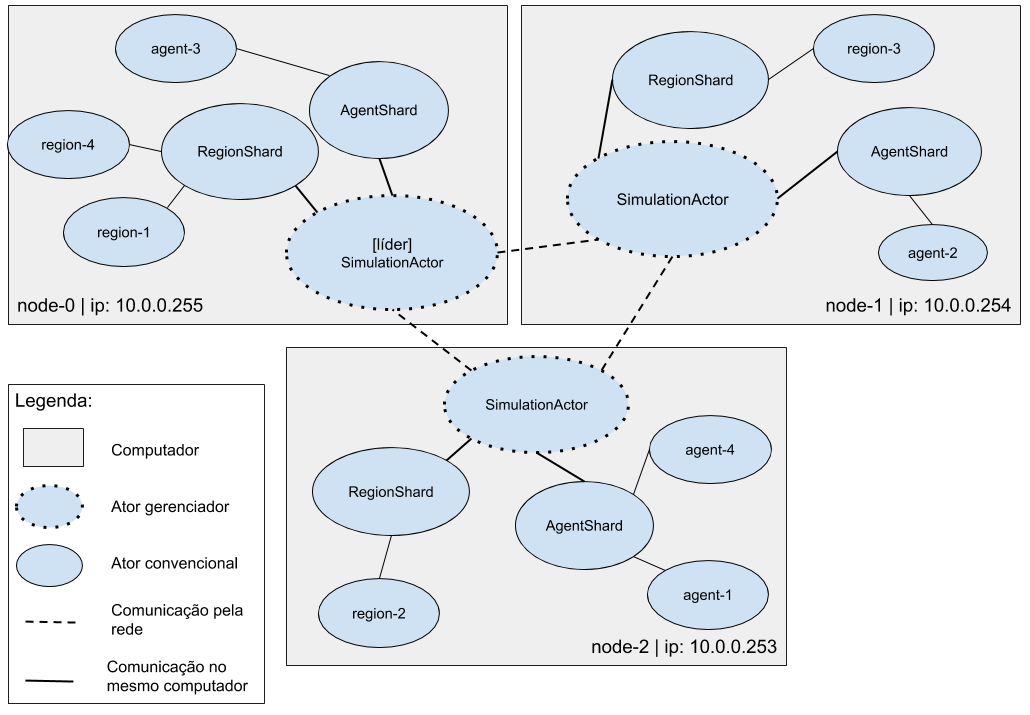
\includegraphics[scale=0.45]{imagens/d-optimas-new.png}
     \fonte{O próprio autor}
     \label{fig:d_optimas_new}
 \end{figure}
 
 A \autoref{fig:d_optimas_new} ilustra a nova organização proposta da arquitetura. Cada ator é representado por uma elipse, os responsáveis por gerenciar a simulação tem a borda pontilhada, e os agentes e regiões, por sua vez, têm as bordas contínuas. As linhas contínuas indicam que os atores se comunicam no mesmo nó, e as linhas tracejadas indicam que os atores se comunicam através da rede. A imagem exemplifica um \textit{cluster} composto por 3 computadores. 
 
 A arquitetura é agora composta de um único ator supervisor por processo, chamado \textbf{SimulationActor}, responsável por gerenciar tanto as regiões quanto os agentes. Quando um nó começa a executar, este é o primeiro ator a ser criado, e há um único para cada processo em execução. O \textbf{SimulationActor} subscreve nos eventos do \textit{cluster} de novo membro (\textbf{MemberUp}), saída de um membro (\textbf{MemberDown}) e de mudança de líder (\textbf{LeaderChanged}), de modo que ele recebe uma mensagem quando qualquer um desses eventos acontece. Quando um segundo nó começa a executar, ambos recebem uma mensagem de que há um novo membro na simulação. Neste ponto, a biblioteca \textit{akka-cluster} elege um líder. Doravante, sempre que o \textbf{SimulationActor} for mencionado, este deve ser associado imediatamente com o líder da simulação, e caso seja necessário falar de um outro ator do mesmo tipo em um nó qualquer, essa distinção será feita. 
  
 O líder tem um papel importante ao longo da execução da simulação. Dentro da especificação da biblioteca \textit{akka-cluster}, ele é o responsável por tarefas administrativas relacionadas ao \textit{cluster}, como por exemplo permitir a entrada de novos membros ou remover um nó que está em estado inacessível. No caso da simulação do D-Optimas, o \textbf{SimulationActor} também é o responsável por iniciar e finalizar a simulação, criar e destruir regiões e manter os agentes atualizados sobre o estado do espaço de busca. Ele também mantém dados estatísticos das regiões, que serão detalhados na seção a seguir. 
 
Ao longo do texto pode parecer que o líder tem um papel crítico na execução da simulação, e que isso pode caracterizar algum tipo de gargalo, ponto único de falha ou controle central. Entretanto, o líder exerce fundamentalmente um papel de coordenador, podendo inclusive ser mudado ao longo da simulação. Executar algumas das tarefas no líder é uma mera questão de escolha, por ser uma maneira mais simples de implementar um algoritmo num ambiente distribuído, sem a adoção um controle central. Isso tão pouco caracteriza um controle central, pois caso um líder fique inoperante, outro nó assume a liderança quase que imediatamente, sem causar prejuízo ou interrupção da simulação. Este comportamento já é um importante passo dado na direção de promover um sistema resiliência a falhas, desde  que seja possível restaurar os agentes/regiões que estavam subordinados ao nó falho. 
 
 Como foi dito, para cada processo criado há um único ator do tipo \textbf{SimulationActor}, que supervisona outros dois atores, o \textit{\textbf{agentShard}} e o \textit{\textbf{regionShard}}. Um ator do tipo \textit{\textbf{Shard}}, disponibilizado na biblioteca \textit{akka-sharding}, um sub-pacote do \textit{akka-cluster}, é o responsável por oferecer transparência de localidade dentro de um \textit{cluster}. Isso permite que os agentes e regiões  troquem mensagens pelo seu endereço lógico, em geral, o nome do ator, em detrimento de seu endereço completo. Caso o \textit{agent-1} queira enviar uma mensagem para a \textit{region-4}, essa mensagem é enviada juntamente com o identificador do destinatário à \textit{shard} mais próxima, que sabe como encaminhar a mensagem ao destinatário. 
 
 Além da transparência de localidade, a biblioteca \textit{akka-sharding} oferece persistência aos atores, utilizando um banco de dados interno e distribuído, baseado em CRDTs (\textit{Conflict-free Replicated Data Types})\cite{shapiro2011}. Isso permite que atores migrem de um \textit{Shard} para outro, caso o primeiro nó esteja mais sobrecarregado que o segundo. A utilização do banco de dados distribuído também permite que, caso um nó falhe, os agentes e regiões sejam restaurados em outro nó, no último estado registrado no banco. Portanto, a arquitetura possui neste ponto algum nível de resiliência a falhas, e também o balanceamento de carga entre os nós. 
 

 
\section{Da dinâmica do espaço de busca e interações entre regiões e o SimulationActor}
\label{sec:dinamica}
% procedimento de inserir uma nova solução
Uma vez construído o sistema, com os agentes e regiões comunicando entre si por meio dos \textit{shards} e conectados ao líder da simulação com auxílio do \textit{akka-cluster}, o próximo passo é entender o comportamento das regiões no sistema. São quatro os algoritmos associados à essa dinâmica: a criação de novas regiões, a inserção de uma solução em uma região, a fissão de uma região e a fusão de duas regiões. 

O primeiro cenário que será abordado é quando um agente produz a primeira solução do sistema e quer enviá-la à uma região. Como o agente tem um conhecimento parcial do mundo, ele sempre envia essa solução para o ator gerenciador da simulação. Sendo as regiões conjuntos não-vazios de soluções, a simulação não possui nenhuma região até que a primeira solução seja criada. O \textit{SimulationActor} é o responsável por criar esta nova região que abrigará aquela solução. Para criar uma região, o \textit{SimulationActor} envia uma mensagem do tipo \textbf{CreateRegion} ao \textbf{RegionShard} subordinado a ele. Internamente, o \textit{akka-cluster} decide em qual nó da simulação essa região vai ser criada, não sendo necessariamente no mesmo nó. Essa decisão será tomada com base no balanceamento das \textbf{Shards}. Uma nova região é criada para cada nova solução recebida até que o sistema atinja o número mínimo de regiões em toda a simulação, que é um parâmetro de configuração do sistema fornecido pelo usuário no arquivo de configuração da simulação. Quando atingido esse limite mínimo, o sistema passa a escolher aleatoriamente a região que receberá a próxima solução.

Esse procedimento aleatório se repetirá até que as regiões tenham pelo menos duas soluções. A partir desse momento, o \textbf{SimulationActor} passa a manter alguns dados relativos às regiões, que são: o valor médio, a variância e o coeficiente de variação das funções objetivo de todas as soluções, bem como o número de soluções para cada região. As fórmulas para o cálculo de cada um desses parâmetros estão descritas na \autoref{tab:formulas}. Ele também agrega os dados de cada região para calcular a estatística global do sistema, que compreende a média, desvio padrão e o coeficiente de variação dos valores de função objetivo de todas as soluções existentes, aqui denotados por $\bar{x}_g$, $s_g$ e $CV_g$, respectivamente.

No momento em que cada região tem ao menos duas soluções e o $CV$ de todas as regiões é diferente de zero, para cada nova solução recebida, o \textbf{SimulationActor} sorteia a região que receberá a próxima solução baseado no coeficiente de varição das regiões: regiões com maior $CV$ tem menor probabilidade de receber soluções, enquanto regiões com menor $CV$ tem chances maiores chances de serem escolhidas. Quando uma região recebe uma solução, ela envia uma mensagem do tipo \textbf{UpdateRegionSummary} para o líder, que atualiza a estatística da região, recalcula a estatística global e envia-a para todas as regiões, através de uma mensagem \textbf{UpdateGlobalSummary} contendo os valores de $\bar{x}_g$, $s_g$ e $CV_g$. 

Sempre que o \textbf{SimulationActor} recebe uma nova solução ele também incrementa um contador, que é considerado o tempo discreto da simulação. Esse tempo é propagado para todos os elementos do \textbf{cluster}, incluíndo os agentes e regiões, utilizando a estratégia de \textit{pig backing} sobre a mensagem de \textbf{UpdateGlobalSummary}. Apesar de funcionar como um relógio lógico global  \cite[p. 244]{tanenbaum}, o tempo discreto não tem o objetivo de criar qualquer mecanismo de sincronização entre os membros da simulação. As mensagens que transmitem soluções são marcadas com esse tempo que é utilizado posteriormente para forçar uma ordenação parcial entre os eventos, facilitando a extração e analise de dados. 

\begin{table}[]
    \centering
    \renewcommand{\arraystretch}{1.5} % Default value: 1
    \caption{Fórmulas utilizadas para calcular os parâmetros de uma região $r$ com $n$ soluções $x_i$, e uma função objetivo é $f(\cdot)$ }
    \label{tab:formulas}
    \begin{tabular}{cc}
        \toprule
         \textbf{Parâmetro} & \textbf{Fórmula} \\
         \midrule
         \\
         Média ($\bar{x}$) & \( \displaystyle \sum_{i = 1}^{i \leq n} f(x_i) \) \\ \\
         Variância ($s^2$) & \( \displaystyle \frac{1}{n - 1} \sum_{i = 1}^{i \leq n} (\bar{x} - f(x_i))^2 \) \\ \\
         Coeficiente de variação ($CV$) & \( \displaystyle \frac{s}{\bar{x}} \) \\ \\
         \bottomrule
    \end{tabular}
\end{table}

No que diz respeito à estratégia de escolha das regiões baseada no $CV$, há outras diferentes formas de se fazer essa escolha, \textit{e.g.} sortear aleatoriamente uma região para receber uma solução. Entretanto, o presente trabalho não pretende avaliar o mérito de uma estratégia, ou comparar esta com qualquer outra. O sorteio probabilístico foi escolhido por ser um algoritmo simples, mas não trivial. O algoritmo proposto não oferece nenhuma garantia sobre como a adição de uma nova solução a uma região particular afetará a distribuição dos valores de função objetivo, podendo fazer essa região tanto se tornar mais especializada, com o $CV$ menor, menos especializada, aumentando  o $CV$. A única premissa do procedimento adotado é que regiões muito especializadas tem mais chances de crescerem em quantidade de soluções. 

% dinâmica interna
As regiões, apesar de não escolherem quais soluções receberão, tem autonomia para se particionar ou se fundir, sendo assim entidades ativas do sistema. Como atores da plataforma \textit{akka} são entidades reativas que somente respondem a mensagens, que podem ter sido enviadas por um outro ator ou pelo próprio receptor, foi utilizado um artifício já proposto por \citeonline{pacheco}. As regiões recebem uma mensagem chamada \textbf{InternalBehaviour}, que é enviada periodicamente pela própria região. Ao receber essa mensagem, a receptora deve escolher, com uma probabilidade de 50\% entre se separar em três outras regiões ou se fundir com uma outra região.

% split das regiões 

Caso uma região região $r$ escolha fazer a fissão, ela deve se certificar de que  duas condições sejam satisfeitas. A primeira delas é que a região possua um número mínimo de soluções, cujo valor é dado pelo usuário no início da simulação. Esse parâmetro existe para evitar que uma região se particione prematuramente. A segunda condição é que o coeficiente de variação dos valores de função objetivo da região $r$ seja maior que o coeficiente de todas as soluções do sistema, \textit{i.e.},  $CV_r > CV_g$. 

Caso essas duas condições sejam satisfeitas a região $r$ se particionará em outras 3 regiões, a saber, as soluções cujo valor de função objetivo estão abaixo de $\bar{x}_{r} - s_{r}$ (cauda inferior), as soluções que estão acima de $\bar{x}_{r} + s_{r}$ (cauda superior) e as soluções que estão entre $\bar{x}_{r} - s_{r}$ e  $\bar{x}_{r} + s_{r}$, onde $\bar{x}_r$ e $s_r$ são a média e o desvio padrão dos valores de função objetivo das soluções que pertencem a região $r$, respectivamente. 

Ao se particionar, a região envia ao \textit{SimulationActor} uma mensagem do tipo \textit{RegionSplit} contendo dois conjuntos de soluções, as da cauda superior e inferior da distribuição. As soluções do centro da distribuição ficam com a região $r$. Ao receber uma mensagem do tipo, \textbf{SimulationActor} verifica se o número máximo de regiões permitidas no sistema não foi atingido, cria as novas regiões com a soluções recebidas. Caso o número máximo já tenha sido atingido, o sistema redistribui aleatoriamente as soluções entre as regiões já existentes. Esse parâmetro do número máximo de regiões também é fornecido no arquivo de configuração do sistema e é necessário para evitar o crescimento exacerbado do número de regiões, levando o sistema a consumir memória de maneira desordenada. 

% procedimento de merge
Caso a região $r_1$ decida por tentar fazer a fusão, ela enviará uma mensagem do tipo \textbf{MergeRequest} para todas as regiões contendo os seus parâmetros estatísticos. Ao receber uma mensagem desse tipo, uma outra região $r_2$ verifica se a união dos dois conjuntos de solução produzira uma nova região $r_3$ cujo $CV_{r_3}$ é menor do que o parâmetro $CV_{r_2}$. Caso essa condição seja satisfeita, a região $r_2$ responde à região $r_1$ com uma mensagem do tipo \textbf{MergeResponse}. Recebendo a primeira mensagem desse tipo, a região $r_1$ imediatamente envia uma mensagem do tipo \textbf{MergeResult} contendo a sua lista de soluções, e se destrói. Outras regiões que tenham respondido à solicitação de $r_1$ terão suas respostas ignoradas, não causando nenhum prejuízo ao sistema.

\begin{quadro}[ht!]
    \centering
    \caption{Mensagens trocadas na arquitetura D-Optimas}
    \label{tab:mensagens}
    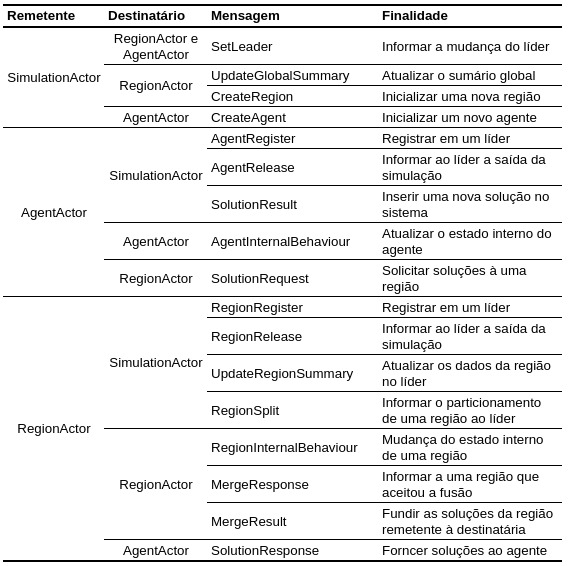
\includegraphics[scale=0.75]{imagens/tabela.jpeg}
    \begin{comment}
\begin{tabular}{lr{2}r{2.5}r{2}}\toprule
\textbf{Remetente} &\textbf{Destinatário} &\textbf{Mensagem} &\textbf{Finalidade} \\\midrule
\multirow{4}{*}{SimulationActor} &RegionActor e AgentActor &SetLeader &Informar a mudança do líder \\
&\multirow{2}{*}{RegionActor} &UpdateGlobalSummary &Atualizar o sumário global \\
& &CreateRegion &Inicializar uma nova região \\
&AgentActor &CreateAgent &Inicializar um novo agente \\
\multirow{5}{*}{AgentActor} &\multirow{3}{*}{SimulationActor} &AgentRegister &Registrar em um líder \\
& &AgentRelease &Informar ao líder a saída da simulação \\
& &SolutionResult &Inserir uma nova solução no sistema \\
&AgentActor &AgentInternalBehaviour &Atualizar o estado interno do agente \\
&RegionActor &SolutionRequest &Solicitar soluções à uma região \\
\multirow{8}{*}{RegionActor} &\multirow{4}{*}{SimulationActor} &RegionRegister &Registrar em um líder \\
& &RegionRelease &Informar ao líder a saída da simulação \\
& &UpdateRegionSummary &Atualizar os dados da região no líder \\
& &RegionSplit &Informar o particionamento de uma região ao líder \\
&\multirow{3}{*}{RegionActor} &RegionInternalBehaviour &Mudança do estado interno de uma região \\
& &MergeResponse &Informar a uma região que aceitou a fusão \\
& &MergeResult &Fundir as soluções da região remetente à destinatária \\
&AgentActor &SolutionResponse &Forncer soluções ao agente \\
\bottomrule
\end{tabular}
\end{comment}
\end{quadro}

O \autoref{tab:mensagens} apresenta um resumo de mensagens do sistema, bem como a finalidade de cada mensagem. 

\section{Do mecanismo de memória Q-learning}

% o que é o q-learning
% qual o modelo básico de atualização da tabela q-learning
% como esse modelo foi adaptado para funcionar com valores de função objetivo 
% como o agente utiliza a memória

\section{Adição de novos algoritmos populacionais}
\label{sec:algoritmos}

Um princípio fundamental na construção da arquitetura D-Optimas é de que a diversidade de estratégias de busca pode, não só levar a arquitetura a encontrar soluções de maior qualidade, quanto melhorar o desempenho geral em diferentes tipos de problema. A cada nova versão da arquitetura, alguns novos algoritmos foram adicionados, em especial na versão de \citeonline{denise2014}, que adicionou vários algoritmos construtores e de busca local. Entretanto, pouco esforço foi empreendido na adição de algoritmos evolutivos ou populacionais, técnica consolidada para solução de problemas complexos, dos quais a única premissa necessária é a de localidade fraca \cite{gaspar2012}.

Neste sentido, fez-se um esforço no presente trabalho de trazer ao menos mais duas técnicas populacionais/evolutivas à arquitetura, de modo que pudessem ser conduzidos experimentos para avaliar o efeito da diversidade de estratégias de busca, algo que não foi testado em trabalhos passados. Os algoritmos inseridos foram o \textit{Differential Evolution} (\textbf{DE}) \cite{storn1997} e o \textit{Particle Swarm Optimization} (\textbf{PSO}) \cite{eberhart1995, eberhart1998}. O algoritmo DE foi escolhido principalmente pela sua simplicidade, uma vez que possui poucos parâmetros de configuração. Por sua vez, o PSO foi escolhido por ser um dos algoritmos de otimização mais citados na literatura, tendo sido aplicado com sucesso em diversos problemas de otimização contínua \cite{bonyadi2017}. 

Ambos os algoritmos foram implementados somente para o problema de otimização irrestrita de função real, para o qual esses algoritmos foram inicialmente propostos. Entretanto, ambos foram implementados usando o arcabouço de generalização proposto por \citeonline{denise2014}, o que torna fácil a extensão deles para problemas de natureza combinatória, bastando implementar os modificadores adequados. Os parágrafos a seguir apresentam os pseudocódigos das estratégias de busca e como eles foram implementados e adaptados para a arquitetura D-Optimas, utilizando os mecanismos de generalização. 

\begin{figure}[ht!]
    \centering
    \caption{Diagrama das estruturas abstratas proposta por \citeonline{denise2014} e como elas foram  utilizadas na implementação dos algoritmos já existentes na arquitetura. As estruturas Problema, Solução e Analise de Solução são comuns a todas implementação de metaheurística. As siglas RMS e RMCS significam, respectivamente, as estruturas de Realiza Modificação de Solução e Realiza Modificação de Conjunto de Solução. São as principais estruturas utilizadas no presente trabalho para implementação dos algoritmos escolhidos. }
    \label{fig:denise_abstract_structures}
    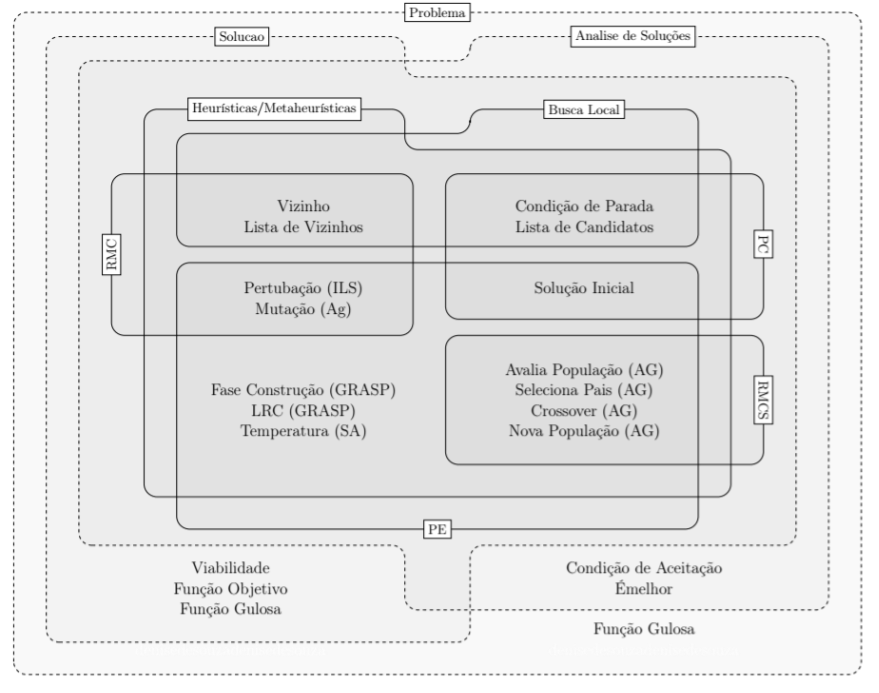
\includegraphics[scale=0.5]{imagens/denise-abstract-structures.png}
\end{figure}

Como já abordado no capítulo anterior \citeonline{denise2014} criou um conjunto de classes abstratas para implementar algoritmos de otimização que sejam independentes dos dados do problema, bem como da representação das soluções. A \autoref{fig:denise_abstract_structures} apresenta essas estruturas abstratas e suas relações com os algoritmos já implementados na arquitetura. Um exemplo é o \textit{Genetic Algorithm} (\textbf{GA}), que utiliza a estrutura de Modificador de Conjunto de Soluções (RMCS) para encapsular a avaliação da população, a seleção dos pais, o cruzamento e a seleção da nova população. 

Portanto, para incluir um novo algoritmo utilizando essas ferramentas foi necessário estudá-las e identificar em cada algoritmo quais os pontos em comum que poderiam depender de um problema específico e encapsulá-los na estrutura apropriada. Deste modo, serão apresentados à seguir os pseudocódigos dos dois algoritmos selecionados, do \textbf{DE} e do \textbf{PSO}, a ideia central da metaheurística e quais trechos foram encapsulados em estruturas abstratas.

A primeira metaheurística abordada será o \textbf{DE}, cujo pseudocódigo é apresentado no \autoref{algo:de}. Essencialmente o algoritmo aplica uma regra simples de seleção e mutação em cada indivíduo da população, sucessivamente, até que uma condição de parada seja atingida. Na implementação original uma população inicial é gerada aleatoriamente. Esse passo foi substituído, evidentemente, pelo comportamento padrão dos agentes na arquitetura que é solicitar um conjunto de soluções às regiões (linha 1). A condição de parada (linha 2) segue o padrão das outras implementações na arquitetura D-Optimas, e é informada pelo usuário no arquivo de configuração da simulação. Há atualmente algumas condições de parada implementadas na arquitetura que estendem a classe abstrata \textbf{StopCondition}. As implementações possíveis são a parada por número máximo de iterações, número máximo de iterações sem melhora, valor da melhor avaliação de função objetivo, tempo máximo de execução ou uma combinação qualquer das condições anteriores. 

A classe \textbf{DE} é composta de dois modificadores, o primeiro responsável por sortear os indivíduos para o cruzamento, o que corresponde a linha 4 do pseudocódigo, e o segundo corresponde a regra de mutação. Como esse modificador recebe uma lista de soluções, que é a população atual, e retorna uma lista contendo três soluções, este modificador é do tipo \textbf{ModifiesSolutionCollection}. O componente recebeu o nome de \textbf{DERandSelection}. 

\begin{algorithm}[H]
\caption{Evolução Diferencial}
\label{algo:de}
\begin{algorithmic}[1]
    \State{$t \gets 1$}
    \State \text{Recebe uma população inicial $X_t$ de tamanho $n$ e dimensão $D$} 
    \While{Condição de parada não for atingida} 
        \For{$i \gets 1$ até $n$} 
            \State{Sorteie $r_1, r_2, r_3 \in {1,\dots,n}$} 
            \State{Sorteie $i_{rand} \in {1, \dots, n}$}
            \For{$j \gets 1$ até $D$}
                \If{$rand(0,1) \leq CR \lor i = i_{rand}$}
                    \State{$u_{t,i,j} = x_{t,i,r_3} + F * (x_{t,i, r_1} - x_{t,i,r_2})$}
                \Else
                    \State{$u_{t,i,j} = x_{t,i,j}$}
                \EndIf
            \EndFor
        \EndFor
        
        \For{$i \gets 1$ até $n$}
            \If{$f(u_{t,i}) < f(x_{t,i})$}
                \State{$x_{t+1,i} \gets u_{t,i}$}
            \Else
                \State{$x_{t+1,i} \gets x_{t,i}$}
            \EndIf
        \EndFor
        \State{$t \gets t + 1$}
    \EndWhile
\end{algorithmic}
\end{algorithm}

As linhas 6 à 12 do \textbf{DE} foram encapsuladas em o segundo modificador de conjunto de soluções, que recebe uma lista contendo quatro soluções e aplica a regra de mutação descrita no algoritmo. Esse modificador foi implementado na classe  \textbf{DEMutationMSC}. 

Há algumas variações para as regras de seleção e mutação do algoritmo \textbf{DE}, que podem ser expressas de uma maneira sintética, de acordo com \citeonline{gaspar2012}. A variação implementada foi \texttt{DE/rand/1/bin}. Entretanto, outras variações podem ser facilmente implementadas sem grandes modificações da classe \textbf{DE}, simplesmente provendo novos modificadores.

A implementação do \textbf{DE} apresenta muito menos desafios do que o algoritmo \textbf{PSO}, cujo pseudocódigo é apresentado no \autoref{algo:pso}. O primeiro problema é a manutenção de duas populações, um vetor de posições que são as soluções do problema de otimização, e uma segunda população que são os vetores de velocidades associados às posições. O comportamento básico do algoritmo é atualizar, a cada iteração, o vetor de velocidade de cada partícula e logo em seguida atualizar a posição até que uma condição de parada seja atingida. Novamente, foi utilizada a estrutura abstrata de \textbf{StopCondition}, cuja implementação concreta é informada no arquivo de configuração da simulação. Para isso, o algoritmo além de receber as soluções iniciais das regiões (linha 1), gera um conjunto de soluções do mesmo tamanho que o primeiro conjunto e inicializa todas aleatoriamente chamando o método \textit{generateInitialSolution()}, definido na classe abstrata \textbf{Solution}. Novamente, foi utilizada a condição de parada genérica \textbf{StopCondition}, cujo tipo concreto é informado no arquivo de configuração da simulação. 

\begin{algorithm}[H]
\caption{Otimização por Enxame de Partículas}
\label{algo:pso}
\begin{algorithmic}[1]
    \State \text{Recebe uma população inicial $X$ de tamanho $n$ e dimensão $D$} 
    \State \text{Gere um conjunto de soluções aleatórias $V$ de tamanho $n$ e dimensão $D$}
    
    \While{Condição de parada não for atingida} 
        \For {$i \gets 1$ até $n$}
            \If{$f(x_i) < f(pb_i)$}
                \State $pb_i \gets x_i$ 
            \EndIf
            
            \If{$f(x_i) < f(gb)$}
                \State $gb \gets x_i$
            \EndIf
        \EndFor
    
        \For {$i \gets 1$ até $n$}
            \For{$d \gets 1$ até $D$}
                \State{$v_{i,d} \gets v_{i,d} + C_1 * rand(0, 1) * (pb_{i,d} - x_{i,d}) + C_2 * rand(0, 1) * (gb_d - x_{i,d}) $}
                \State{$x_{i,d} \gets x_{i,d} + v_{i,d}$}
            \EndFor
        \EndFor
    \EndWhile
\end{algorithmic}
\end{algorithm}

O algoritmo mantém uma terceira lista de soluções que armazena a melhor posição de cada indivíduo do enxame ao longo da execução do algoritmo, que corresponde no pseudocódigo à variável $pb_i$. Além desta memória, ele também mantém melhor partícula ao longo da execução, que corresponde à variável $gb$. A cada iteração essas variáveis são atualizadas, e para fazer a comparação, utilizamos a classe abstrata  \textbf{SolutionAnalizer}, que fornece métodos para efetuar a comparação entre duas soluções. Essa classe deve ser estendida e o seu tipo concreto também é informado no arquivo de configuração. 

Os passo de alteração dos vetores velocidade e posição foram implementados em dois modificadores de coleção diferentes. Para modificar as velocidades, é necessário passar um vetor de tamanho $2*n + 1$, contendo nas $n$ primeiras posições os vetores de velocidade, nas $n$ posições seguintes o vetor $pb$ e na última posição da lista a melhor solução até a t-ésima iteração $gb$. Esse modificador foi nomeado \textbf{PSOVelocityUpdateMSC} e corresponde a linha 14 do \autoref{algo:pso}. Por fim, o modificador \textbf{PSOPositionUpdateMSC} recebe uma lista de tamanho $2n$ contendo nas $n$ primeiras posições o vetor $X$ e nas $n$ posições seguintes o vetor V  atualiza a lista de posições, encapsulando a linha 15 do pseudocódigo.

\section{Considerações finais}
O presente capitulo se dedicou a apresentar as alterações feitas na arquitetura D-Optimas, proposta inicialmente por \citeonline{pacheco}. Essas alterações tiveram o principal objetivo de melhorar aspectos teóricos e evoluir a arquitetura, por exemplo, conferindo resiliência à simulação, do ponto de vista de sistemas distribuídos e dando uma definição precisa para o comportamento das regiões. Foram adicionadas também mais estratégias de busca, para cumprir o propósito da D-Optimas, como um sistema multi-agente, onde há diversidade de estratégias.

O capitulo seguinte apresentará alguns experimentos preliminares para avaliar as mudanças que foram feitas até o momento, principalmente no que diz respeito ao desempenho computacional e a escalabilidade da arquitetura.